\documentclass[tikz,border=4pt]{standalone}
\usepackage{pgfplots}
\pgfplotsset{compat=1.16}
% un colore per ogni Q, gli stessi in tutti i diagrammi del secondo ordine
\colorlet{Q1}{orange}              % Q = 1
\colorlet{Q2}{magenta}             % Q = 2
\colorlet{Q5}{black}               % Q = 5
\colorlet{Q10}{cyan!70!black}      % Q = 10
\pgfplotsset{
  bode/.style={
    width=6.4cm, height=4.4cm, xmin=0.01, xmax=100,
    grid=both, major grid style={gray!55}, minor grid style={gray!20},
    tick label style={font=\footnotesize}, label style={font=\small},
    title style={font=\small}, xlabel={$\omega/\omega_u$},
  },
  bode mag/.style={bode, ymin=-50, ymax=50, ytick={-40,-20,0,20,40},
    ylabel={$|H|_{\mathrm{dB}}$}, title={Modulo}},
  bode fase/.style={bode, ymin=-100, ymax=100, ytick={-90,-45,0,45,90},
    ylabel={$\varphi$ [$^\circ$]}, title={Fase}},
}
\begin{document}
% Sallen-Key passa-banda:  H(j w) = G0 / (1 + j Q (x - 1/x)),  x = w/w0
% Modulo normalizzato a G0 (0 dB al centro banda):
%   |H/G0|_dB = -10 log[1 + Q^2 (x - 1/x)^2],   fase = -atan[Q (x - 1/x)]
% Per il guadagno vero basta sommare 20 log(3Q-1) al modulo (G0 = 3Q-1 nella struttura della lezione).
% Punti a -3 dB:  x1,2 = sqrt(1 + 1/(4Q^2)) -/+ 1/(2Q)   ->   B = f0/Q
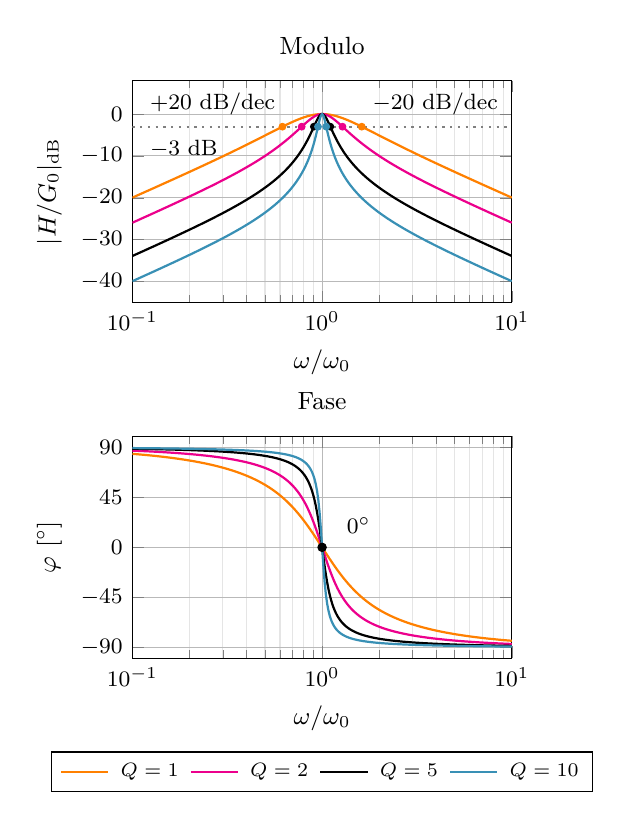
\begin{tikzpicture}
% ---------- modulo ----------
\begin{semilogxaxis}[bode mag, name=mag, xmin=0.1, xmax=10, xlabel={$\omega/\omega_0$},
  ylabel={$|H/G_0|_{\mathrm{dB}}$}, ymin=-45, ymax=8, ytick={-40,-30,-20,-10,0}]
  \addplot[gray, dotted, thick, forget plot] coordinates {(0.1,-3.01) (10,-3.01)};
  \addplot[Q1, thick, domain=-1:1, samples=301]
    ({10^x}, {-10*log10(1+(1*(10^x-10^(-x)))^2)});
  \addplot[only marks, mark=*, mark size=1.2pt, Q1, forget plot] coordinates {(0.6180,-3.01) (1.6180,-3.01)};
  \addplot[Q2, thick, domain=-1:1, samples=301]
    ({10^x}, {-10*log10(1+(2*(10^x-10^(-x)))^2)});
  \addplot[only marks, mark=*, mark size=1.2pt, Q2, forget plot] coordinates {(0.7808,-3.01) (1.2808,-3.01)};
  \addplot[Q5, thick, domain=-1:1, samples=301]
    ({10^x}, {-10*log10(1+(5*(10^x-10^(-x)))^2)});
  \addplot[only marks, mark=*, mark size=1.2pt, Q5, forget plot] coordinates {(0.9050,-3.01) (1.1050,-3.01)};
  \addplot[Q10, thick, domain=-1:1, samples=301]
    ({10^x}, {-10*log10(1+(10*(10^x-10^(-x)))^2)});
  \addplot[only marks, mark=*, mark size=1.2pt, Q10, forget plot] coordinates {(0.9512,-3.01) (1.0512,-3.01)};
  \node[anchor=north west, font=\footnotesize] at (axis cs:0.11,7.5) {$+20$ dB/dec};
  \node[anchor=north east, font=\footnotesize] at (axis cs:9.5,7.5) {$-20$ dB/dec};
  \node[anchor=north west, font=\footnotesize] at (axis cs:0.11,-3.8) {$-3$ dB};
\end{semilogxaxis}
% ---------- fase ----------
\begin{semilogxaxis}[bode fase, at={(mag.south west)}, yshift=-1.7cm, anchor=north west,
  xmin=0.1, xmax=10, xlabel={$\omega/\omega_0$},
  legend columns=4, legend style={font=\scriptsize, at={(0.5,-0.42)}, anchor=north, column sep=2pt},
  legend cell align=left]
  \addplot[Q1, thick, domain=-1:1, samples=301]
    ({10^x}, {-atan(1*(10^x-10^(-x)))});
  \addlegendentry{$Q=1$}
  \addplot[Q2, thick, domain=-1:1, samples=301]
    ({10^x}, {-atan(2*(10^x-10^(-x)))});
  \addlegendentry{$Q=2$}
  \addplot[Q5, thick, domain=-1:1, samples=301]
    ({10^x}, {-atan(5*(10^x-10^(-x)))});
  \addlegendentry{$Q=5$}
  \addplot[Q10, thick, domain=-1:1, samples=301]
    ({10^x}, {-atan(10*(10^x-10^(-x)))});
  \addlegendentry{$Q=10$}
  \addplot[only marks, mark=*, mark size=1.5pt, black, forget plot] coordinates {(1,0)};
  \node[anchor=south west, font=\footnotesize] at (axis cs:1.2,4) {$0^\circ$};
\end{semilogxaxis}
\end{tikzpicture}
\end{document}
